% Copyright (c) 2008, João Henrique Ferreira de Freitas
% All rights reserved.
% 
% Redistribution and use in source and binary forms, with or without modification,
% are permitted provided that the following conditions are met:
% 
%     * Redistributions of source code must retain the above copyright notice,
%       this list of conditions and the following disclaimer.
%     * Redistributions in binary form must reproduce the above copyright notice,
%       this list of conditions and the following disclaimer in the documentation and/or 
%       other materials provided with the distribution.
%     * Neither the name of the <ORGANIZATION> nor the names of its contributors may
%       be used to endorse or promote products derived from this software without 
%       specific prior written permission.
% 
% THIS SOFTWARE IS PROVIDED BY THE COPYRIGHT HOLDERS AND CONTRIBUTORS "AS IS" AND ANY 
% EXPRESS OR IMPLIED WARRANTIES, INCLUDING, BUT NOT LIMITED TO, THE IMPLIED WARRANTIES
% OF MERCHANTABILITY AND FITNESS FOR A PARTICULAR PURPOSE ARE DISCLAIMED. IN NO EVENT
% SHALL THE COPYRIGHT OWNER OR CONTRIBUTORS BE LIABLE FOR ANY DIRECT, INDIRECT, INCIDENTAL,
% SPECIAL, EXEMPLARY, OR CONSEQUENTIAL DAMAGES (INCLUDING, BUT NOT LIMITED TO, PROCUREMENT
% OF SUBSTITUTE GOODS OR SERVICES; LOSS OF USE, DATA, OR PROFITS; OR BUSINESS INTERRUPTION)
% HOWEVER CAUSED AND ON ANY THEORY OF LIABILITY, WHETHER IN CONTRACT, STRICT LIABILITY,
% OR TORT (INCLUDING NEGLIGENCE OR OTHERWISE) ARISING IN ANY WAY OUT OF THE USE OF THIS
% SOFTWARE, EVEN IF ADVISED OF THE POSSIBILITY OF SUCH DAMAGE.
% 
% $Id$

\section{Materiais e Métodos} \label{sec:materiais}

%Nesta seção discorreremos sobre como a pesquisa foi elaborada 

Existem várias razões para um usuário colaborar com um projeto de SL/CA. Razões ideológicas, técnicas e necessidades de novas funcionalidades para resolver seus problemas são as mais comuns. Consequentemente, a colaboração ou patch\footnote{Patch pode ser definido como sendo uma mudança, conserto ou melhoramento. Incluindo código fonte e documentação. É parte do processo de desenvolvimento SL/CA e muitos projetos possuem guias que descrevem os requisitos para a submissão do patch mas poucos utilizam um processo de revisão e aprovação.\cite{preliminary}}) visam melhoramentos na documentação, suporte a lista de discussão, codificação, manutenção de código e testes. Para todas as contribuições que o usuário pretende fazer, existe um caminho pré suposto no qual se refere aos processos necessários para a colaboração se tornar realmente efetiva no projeto. Um exemplo de uma colaboração não efetiva é a implementação de uma nova funcionalidade que não segue as políticas de codificação e design do projeto em questão, gerando retrabalho ou abandono do trabalho.

Inicialmente destacamos três softwares no qual gostaríamos de contribuir a fim de codificar determinadas funcionalidades desejadas. Os três softwares são relacionados a infraestrutura de redes, a saber: \textit{Pfsense}\footnote{http://www.pfsense.org}: personalização do sistema operacional FreeBSD para atuar como firewall; \textit{Tikiwiki}\footnote{http://www.tikiwiki.org}: software de gerenciamento de contéudo (CMS); \textit{Bacula}\footnote{http://www.bacula.org}: software de gerenciamento de backup em rede. Mediante ao levantamento inicial realizado, apenas um seria escolhido para a experimentação. A escolha foi feita privilegiando o projeto com maior tempo de vida e estabilidade no ciclo de releases.

% TODO: enquadrar e definir o processo
% - De acordo com o autor, processos são compostos por tarefas e ações atômicas. 
% Cada ação é seguida de entidades: 
% -- agentes participantes da atividade
% -- ferramentas utilizadas pelos agentes para a realização das atividades
% -- recursos que são produzidos e necessários para realizar a atividade
% -- scripts ou métodos contendo a descrição da ação
\subsection{Coleta de Dados} \label{subsection:coletadados}

Cada projeto de SL/CA estabalece métodos próprios de interação, comunicação, liderança e controle. Além das informações dentro da comunidade serem dinâmicas, novos artefatos são inclusos, outros apagados ou desatualizados podendo gerar uma certa frustração na investigação inicial. Felizmente existem diversos frameworks \cite{reference} para tratar a diversidade das informações e torná-las mais padronizadas para a análise de processos num ambiente de SL/CA ou proprietário. Como não era o nosso objetivo descobrir todo o processo de software vinculado ao projeto de SL/CA mas sim uma particularidade comum a todos os projetos de SL/CA, que é a contribuição do usuário no desenvolvimento, não seguimos estritamente um framework para definição de processos.

Na pesquisa realizada, para facilitar a análise do processo colaborativo, além de definir a posição observadora, foi necessário utilizar uma classificação (taxionomia\footnote{Ciência da classificação.}) com componentes que formavam o projeto investigado. Partindo do princípio que toda e qualquer informação de um projeto de SL/CA necessita estar publicamente acessível, iniciamos anotando informações disponíveis publicamente na página oficial do projeto. 

Procuramos traços de informações onde poderíamos encontrar detalhes sobre as relações entre tarefas, ações, atividades, agentes, ferramentas, recursos e padrões utilizados na composição do projeto (figura \ref{fig:mapping}). Esta busca foi denominada de ``entendimento do domínio do problema'' \cite{experience}. Alguns dos principais itens incluíram:

% •  Web pages, including project status reports and task assignments, may be viewed
%   and classified (informally) as object types.
% • Asynchronous communications among project participants posted in threaded
%   email discussion lists, which address process activities indicated by process
%   identifier keywords (e.g., design, release, testing, etc.)
% • Transcripts of synchronous communication via Internet chat (cf. [5]).
%   Software problem/bug and issue reports, which reveal information on software
%   bug reporting and maintenance/repair processes
% • Testing scripts and results, which highlight project-based software testing
%   practices
% • Community newsletters, which highlight project milestone events (e.g., system
%   releases, turnover of core developers in the projects)
% • Web accessible software product source code directories and repositories, which
%   carry timestamps and other identifiers indicating when source code objects were
%   checked in/out, and versioning information.
% • Software system builds (executable binaries) and distribution packages, which are
%   constructed and released on a periodic basis (daily, candidate (alpha, beta), and
%   final release (distribution version)
% • OSS development tools in use in an OSSD project (e.g., concurrent version
%   system (CVS), GNU compiler collection (gcc), bug reporting (bugzilla) (cf. [10])
% • OSS development resources, including other software development artifacts and
%   process fragment descriptions (e.g., How-To guides, lists of frequently asked
%   questions (FAQs), etc.) [26]

\begin{itemize}
 \item Páginas web, relatório de status e atribuições de trabalho;
 \item Comunicação assíncrona entre participantes postadas em listas de discussão via email, no qual endereçavam identificadores de processos (isto é, design, release, testing);
 \item Scripts de teste e resultados, sinalizando processos de testes;
 \item Notícias da comunidade, identificando principais acontecimentos (novas releases ou marcos especiais);
 \item Acessibilidade do repositório de código fonte com identificações, timestamps e versionamentos;
 \item Sistemas de build automáticos;
 \item Ferramentas de desenvolvimento SL/CA utilizadas no projeto (controle de versão, compiladores, gerencia de configuração, bug reporting, framework para testes);
 \item Recursos de desenvolvimento, incluindo outros tipos de artefatos, fragmentos descritivos de processos (isto é, guias (howto), listas de perguntas frequentes (FAQs)).
\end{itemize}

\begin{figure}[h]
 \centering
 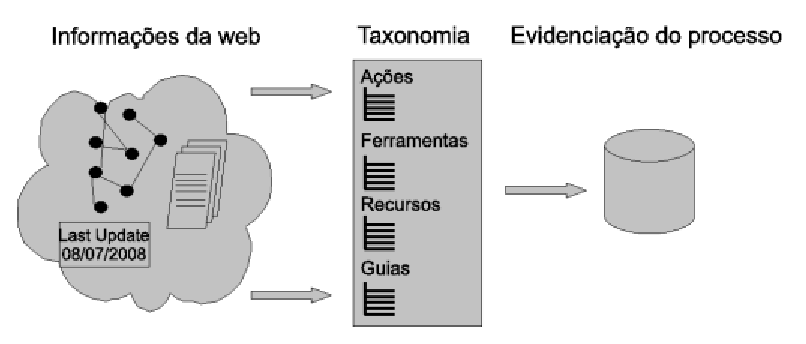
\includegraphics{../../doc/diagramas/maping.eps}
 % maping.eps: -1214733968x146666624 pixel, 300dpi, -10284748.00x1241777.38 cm, bb=0 0 731 292
 \caption[Mapeamento de informações]{Mapeamento de informações, divisão de estruturas e composição de processo \cite{refframework}}
 \label{fig:mapping}
\end{figure}

% - Artefatos comuns: webpages, chats scripts, development resources, process description (howto guides, FAQs)
% 
% - Dimensões dos artefatos: 
% -- Estrutural, how project-related software development artifacts are organizad
% -- Conteudo, tipos de artefatos e informações que eles contém
% -- Pattern de uso, interação do usuário com a comunidade
% -- Pattern de atualização, atualização de conteúdo, criação e remoção

% - Segundo o autor a descoberta do processo específico de um projeto OSSD se inicia com uma exploração no Web space anotando quais informações estão disponíveis e onde podem ser localizadas. Esta exploração nos dá a ideía do que acontece com as ações, agentes, ferramentas e recursos, padrões de utilização a atulização.
% 

Em seguida, classificamos as informações levantadas em três dimensões formadas por:
\begin{itemize}
 \item Estrutural: levantamento de como os artefatos são desenvolvidos e sua organização estrutual;
 \item Conteúdo: levantamentos dos tipos de artefatos e conteúdos;
 \item Padrões de utilização: interação do usuário, desenvolvedores e padrões de atualização com a comunidade.
 \end{itemize}

% The structure of the community Web is evident in two forms. The
% physical form consists of the directory structure of the files of
% which the site is composed. But, it is also apparent on a logical
% level, in terms of the site layout, as might be given by a site map
% or menu. These may or may not be equivalent. Nevertheless,
% each layer in the hierarchy provides a clue to the types of agents,
% resources, tools, and processes of the community. Structure
% hierarchy names may be mapped to instances of tools, agents,
% resources, and activities found in the open source software
% development meta-model taxonomy, thus fulfilling the first role
% of the reference framework.
A organização estrutural da comunidade geralmente é evidente na hierarquia organizacional adotado pelo web site do projeto em função de seu layout e diretórios de acesso. Diretórios com grande número de arquivos e arquivos grandes podem indicar intensa atividade como observado em listas de email e fórums, repositório de código fonte, notícias da comunidades, repositórios de \textit{issue}, seções de release e \textit{ChangeLogs}, entre outras. A presença destes itens indicam um processo de desenvolvimento.

% Additionally, directories with a high
% amount of content, both due to file numbers and file size may
% indicate a focus on activity in that area. Claims such as these may
% then be reinforced or refuted based on additional information
% gathered during discovery. Common to most open source
% communities are mailing lists and discussion forums, source
% repositories, community newsletters, issue repositories, and
% binary release sections, among others. The mere presence of
% these suggests certain activities in the development process.

As relações começam a se tornar mais evidentes quando investigamos o conteúdo do repositório de código fonte e relacionamos com um bugtracker\footnote{É um sistema desenvolvido para ajudar no gerenciamento de bugs a fim de melhorar a qualidade do sistema a ser desenvolvido. Geralmente um bug tracker é uma porção menor de um issue tracker, \url{http://en.wikipedia.org/wiki/Bugtracker}} ou issuetracker\footnote{Issue é uma unidade de trabalho com o objetivo de melhoramento. Pode ser um bug, melhoramento, tarefa, documentação, entre outras. Tradicionalmente issue pode ser traduzido como \textit{problema}, \url{http://en.wikipedia.org/wiki/Issue_tracking_system}}. Esta relação diz como as mudanças no código fonte são realizadas e se há algum processo de teste implantado. Em algumas comunidades o banco de dados de issue também é utilizado para requisitar novas features, enquanto que em outras geralmente encontramos em forums ou listas de discussão. Entretanto iremos encontrar a maioria dos dados relacionados nas páginas web, em mensagens de email, guias gerais e tudo que possa compor um quadro de informações autocontido.


% These also signal what types of data may be contained therein. If
% we just look at source repositories, we can obtain a process
% specification of a limited set of activities- those that involve
% changes to the code, just as issue and bug databases tell us that
% some testing is done on which the issue reports are based. In
% some communities, issue reports are also used to file feature
% requests. Such information may also be found within discussion
% forums or email lists.
% 


% The bulk of the process data is found within the content of Web
% artifacts. Much of the mapping consists of text matching between
% strings in artifacts such as web pages, and email messages and
% process related keywords as was demonstrated for structure-based
% data. In the case of web content, we are also looking for items
% like date stamps on email messages to place the associated events
% in time, document authors, and message recipients. In some
% cases, it is possible to uncover “how-to” guides or partial process
% prescriptions. Like other content, these may not accurately reflect
% the process as it is currently enacted, if they ever did. Therefore,
% each datum must be verified by others.

Padrões de uso são indicadores das principais áreas do espaço web mais ativas, reforçando a validação dos dados encontrados e quais atividades do processo estão ocorrendo em determinado tempo. Podem ser evidenciadas via contadores de acesso e estatísticas de última atualização.

% Usage patterns, like content size, are indicators of which areas of
% the Web space are most active, which reinforces the validity of
% the data found therein and also what activities in the process may
% be occurring at a given time. Web access logs, if available,
% provide a rich source of data. Page hit counters and last update
% statistics are also useful for this purpose. 

% OSSD artifacts vary along these three dimensions over time, and
% this variance is the source of process events. To effectively
% discover processes, our reference framework must be able to
% relate artifacts in the community Web space with process actions,
% tools, resources, and roles.

Artefatos de desenvolvimento SL/CA variam dentro das três dimensões (estrutural, conteúdo, padrões de utilização) durante todo o tempo. A análise se torna mais efetiva quanto mais minuciosa for a classificação executada e o cruzamento dos dados com a engenharia de software tradicional.

% 
% - Em uma organização é possível determinar algumas coisas olhando para um gráfico organizacional e coisas do tipo. Já em um projeto open-source não há este tipo de artefato.
% 
% - O processo de engenharia de requisitos é diferente do tradicional (elicitação, especificação, análise, modelagem, comunicação e gerenciamento)
% 
% 
% 

% - Casos de uso podem ser utilizados para demonstrar as interrealções das ações, utilização de ferramentas e atores. Os casos de uso podem ser integrados para produzirem um conteúdo de hypermedia relacionando todas as atividades do processo.



